\chapter{Technical report}

\section{QT-Robot}
\subsection{Presentation}
\begin{minipage}{.33\textwidth}%
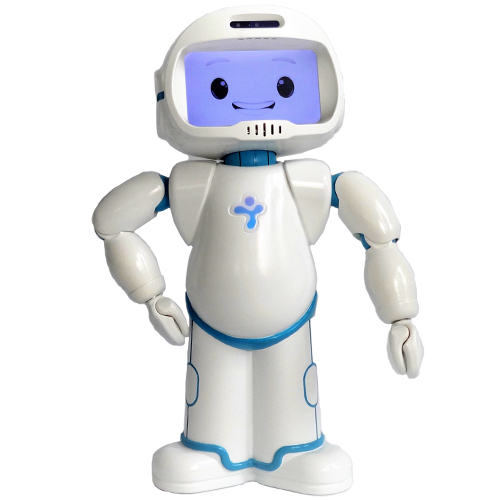
\includegraphics[width=\textwidth]{Figures/qtrobot2.jpg}
\captionof{figure}{QTrobot}
\end{minipage}%
\hfill
\begin{minipage}{.5\textwidth}%
QTrobot is a social robot developed by LuxAI. It has been designed to interact with autistic children and provide them with an interactive learning platform. QTrobot uses artificial intelligence and facial recognition features to engage children in educational and therapeutic activities. It can express emotions, speak, and play interactive games to encourage learning and communication. QTrobot is widely used in schools, autism treatment centers and homes to support the social and emotional development of autistic children.\\
\end{minipage}%

\subsection{Features}

Its operation is based on the integration of several technologies to enable interactions with autistic children, of which we give an overview :\\
\begin{enumerate}

\item Hardware: QTrobot is equipped with various hardware components such as a face screen, speakers, microphones, motion sensors and motors for physical movement.
\\
\item Software: QTrobot uses software based on ROS (Robot Operating System), which provides an infrastructure for managing the robot's functions and interactions. ROS facilitates communication between QTrobot's various hardware and software components.
\\
\item Interaction: QTrobot uses artificial intelligence features to recognize and track faces, detect facial expressions and establish visual communication with children.
\\
\item Communication: QTrobot can speak and understand speech thanks to its voice recognition capabilities. It can also express emotions through its facial display and body movements, enabling it to establish non-verbal communication with children.

\item Educational activities: QTrobot offers interactive educational activities to help autistic children in their learning and development. It can play games, present image sequences, teach social skills, or help with understanding and practicing various tasks.

\item Adaptability: QTrobot is designed to adapt to children's individual needs and preferences. It can be configured to adjust the level of difficulty of activities, the intensity of interactions and the areas of learning targeted.\\
\end{enumerate}

\subsection{Architecture}
 The QTrobot is equipped with state-of-the-art hardware, such as long-range microphones, a 3D camera and powerful computers. The platform is made up of two computers: the QTRP, based on Raspberry Pi and responsible for controlling the main hardware, and the QTPC, an Intel® NUC i5/i7 PC offering enhanced computing power. Both computers run Ubuntu/Debian Linux operating systems and use ROS for their operation.

 \begin{figure}[!h]
\centering
 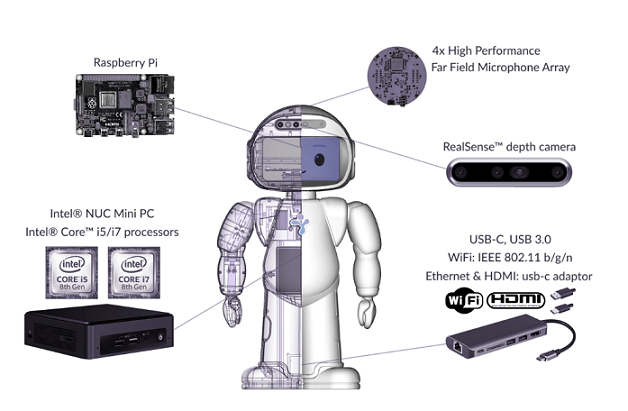
\includegraphics[width=14.25cm]{Figures/qt_architecture.png}
 \caption{QTrobot architecture }
\end{figure}

\begin{minipage}{.55\textwidth}%
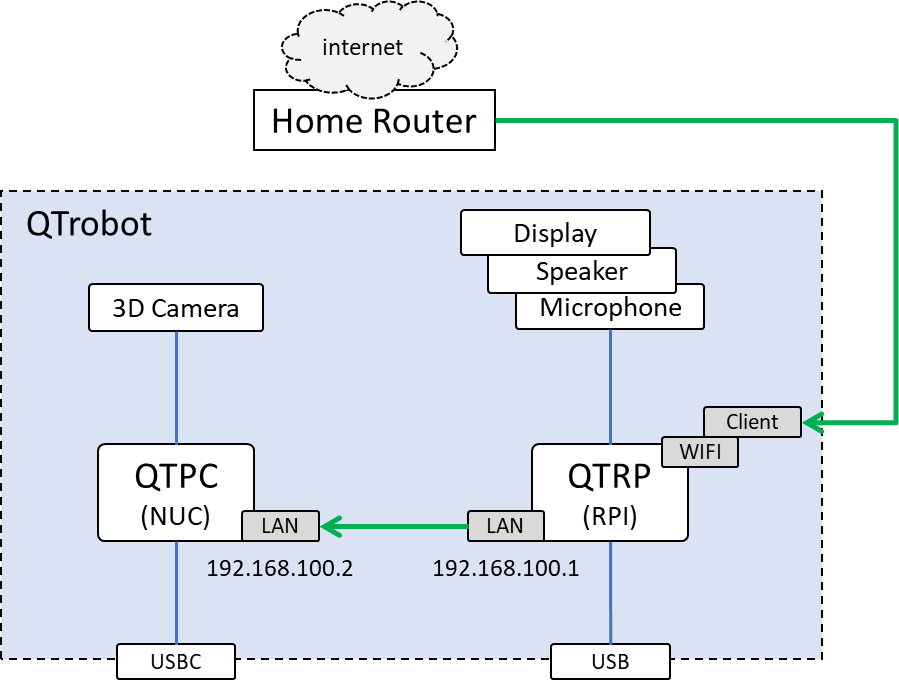
\includegraphics[width=\textwidth]{Figures/qt_network.png}
\captionof{figure}{QTrobot network}
\end{minipage}%
\hfill
\begin{minipage}{.33\textwidth}%
In order to access and use the Internet, we need the QTRP wifi to be connected to a router. The internet will then be shared with all other equipment via QTRP. The green arrow indicates the direction and manner in which the Internet is shared.\\
\end{minipage}%
\vspace*{1.2cm}
\subsection{QT-robot Studio}
We began by familiarizing ourselves with robot programming using QT-robot Studio. This platform enabled us to learn how to use the robot and develop specific programs for its functions. There are also two tablets connected to the QTrobot: an "Educator" tablet and a "Learner" tablet. Once we've completed our script with QTRobot Studio, we transfer it to the Educator tablet. This allows us to modify and add scripts as required. The second tablet, the Learner tablet, plays an important role in the experiments, enabling participants to interact with visuals.\\

 \begin{figure}[!h]
\centering
 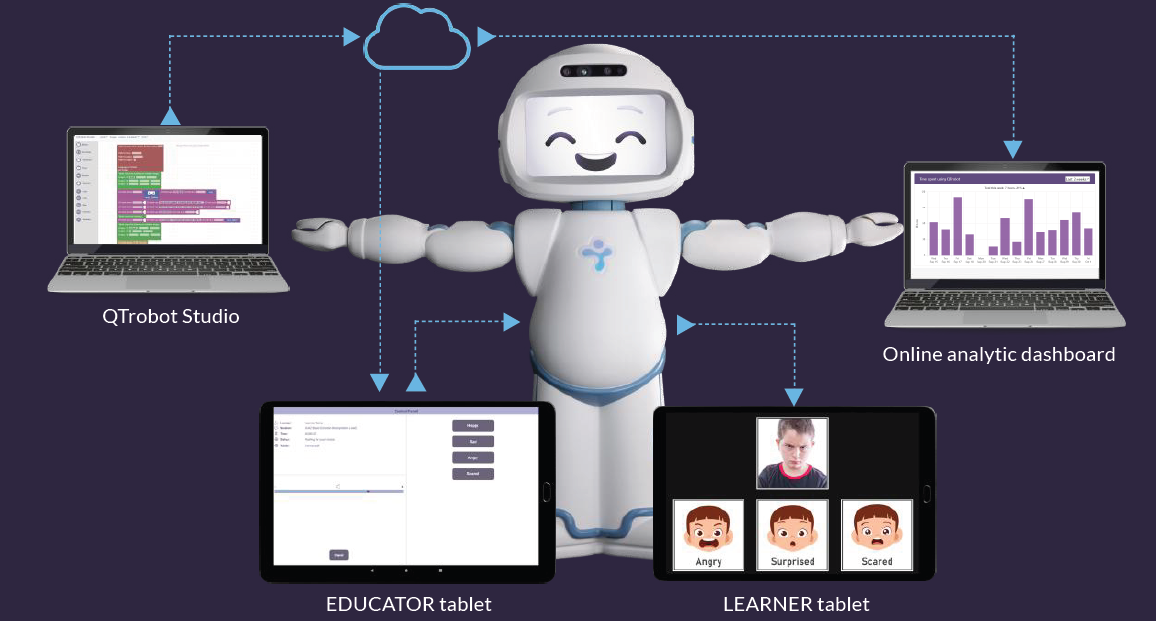
\includegraphics[width=14.25cm]{Figures/qtstudio.png}
 \caption{QT-robot Studio }
\end{figure}
\newpage
We then created a first script in order to be able to communicate briefly with the robot:
 \begin{figure}[!h]
\centering
 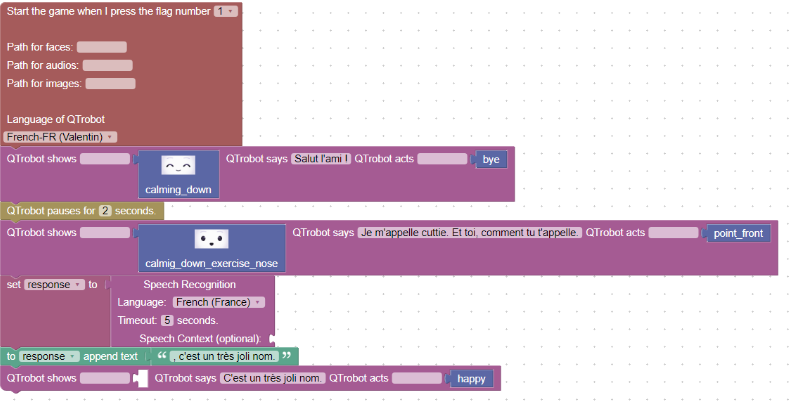
\includegraphics[width=14.25cm]{Figures/qtrobotscript1.png}
 \caption{QTrobot Studio Script}
\end{figure}

\subsection{Working environment}
We explored programming using tablets and QTrobot Studio, also known as "visual scripting". This principle proved interesting to understand and learn, but we also noted certain limitations. Indeed, although QTrobot Studio offers a user-friendly interface for programming, we discovered that certain advanced functionalities are only accessible by using ROS (Robot Operating System) and configuring a keyboard-mouse connection. This means that to fully exploit QTrobot's potential and access all available features, we had to adopt more traditional programming using ROS and interacting with the robot using a keyboard-mouse configuration.
\vspace*{0.5cm}
\subsubsection{Robot Operating System (ROS)}
ROS (Robot Operating System) is an open-source software development framework widely used in the field of robotics. It provides a flexible and robust platform for the creation of advanced robotic systems, enabling communication between hardware and software components.\\
\\
ROS consists of numerous tools, libraries and conventions that simplify software development for robots. It offers features such as message management, node management (computing units), package management (grouping of code and resources) and service management (synchronous communication between nodes).\\
\\
Thanks to its popularity and broad ecosystem, ROS is used in many areas of robotics, from industrial and service robots to research and education. \\

\subsubsection{Keyboard / Mouse}
To make full use of the ROS framework, we had to change the way we use the robot and connect it to a keyboard and mouse.\\
\\
\begin{minipage}{.6\textwidth}%
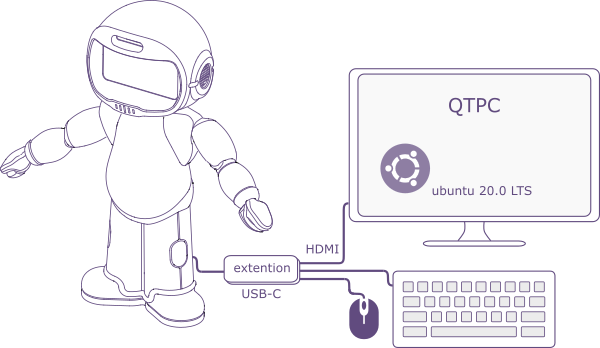
\includegraphics[width=\textwidth]{Figures/qtsourissetup.png}
\captionof{figure}{Setup QTrobot}
\end{minipage}%
\hfill
\begin{minipage}{.33\textwidth}%
Here's the expected configuration: connect the mouse, keyboard and monitor to the robot, then switch on the monitor in the same way as a conventional computer.\\
\end{minipage}%

\subsection{Main scripts}

\subsubsection{Voices}
We then had to learn how to use ROS and all its features to create our script. First, we changed the robot's voice to French to facilitate communication.

\begin{minipage}{.6\textwidth}%
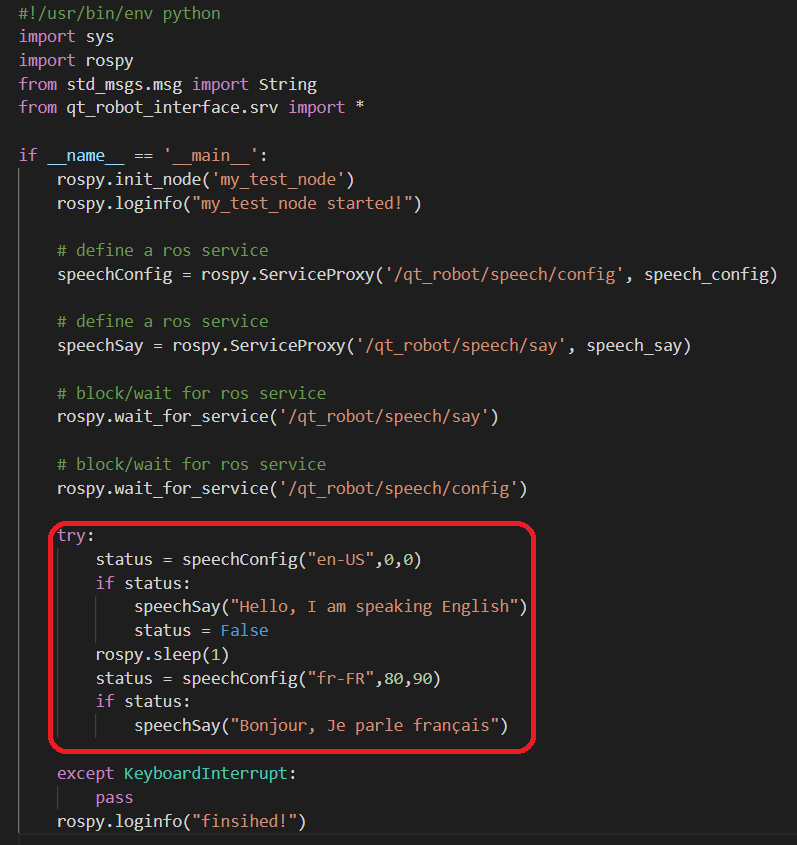
\includegraphics[width=\textwidth]{Figures/qtrobotscript2langue.png}
\captionof{figure}{Python script with french voice}
\end{minipage}%
\hfill
\begin{minipage}{.33\textwidth}%
Here's the script we used to change the language to French. We can see that \textit{speechConfig("fr-FR",80,90)} includes three parameters, the first corresponding to the language, the second to the voice pitch and the third to modify the reading speed.\\
\end{minipage}%

\subsubsection{The game}
To make the discussion as natural as possible, we made the robot pause between sentences.\\
\\
\begin{minipage}{.6\textwidth}%
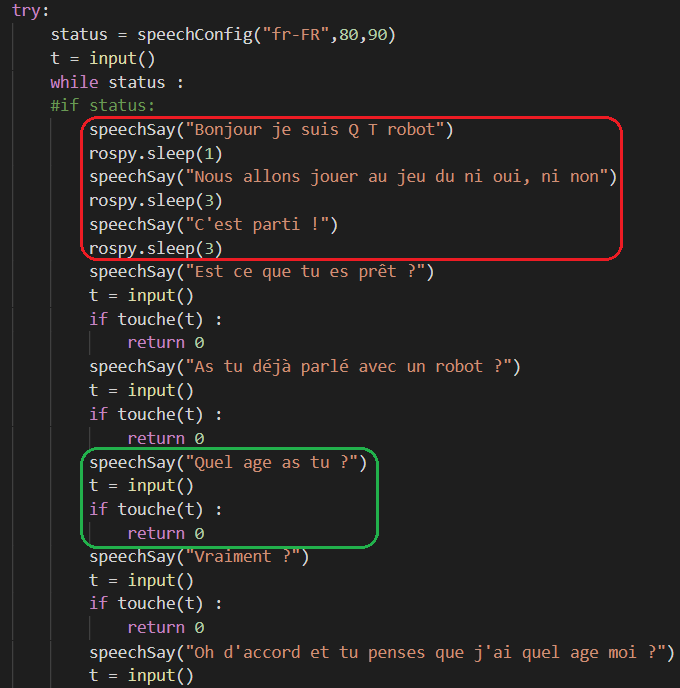
\includegraphics[width=\textwidth]{Figures/qtrobotscript3.2text.png}
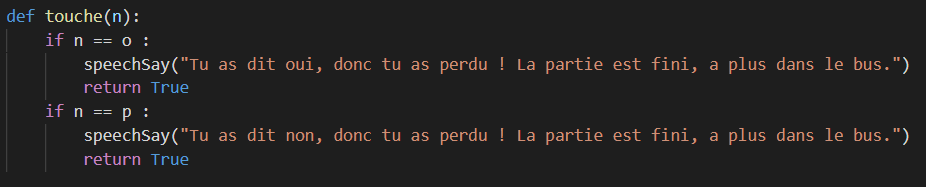
\includegraphics[width=\textwidth]{Figures/qtrobotscript3text.png}
\captionof{figure}{Python script "neither yes nor no"}
\end{minipage}%
\hfill
\begin{minipage}{.33\textwidth}%
 To do this, we first used \textit{rospy.sleep(1)} with the desired time as argument. Next, we created a function \textit{touche(t)} taking as an argument the key pressed by the experimenter.  If the participant answers "yes" or "no", then the key pressed is \textit{o} or \textit{p} respectively, and our function returns a sentence for the loser. Otherwise, the experimenter presses any key to launch the other questions.
\end{minipage}%
\noindent
\subsubsection{Movements}
We've also tried our hand at teaching the robot how to move.\\
\\
\begin{minipage}{.6\textwidth}%
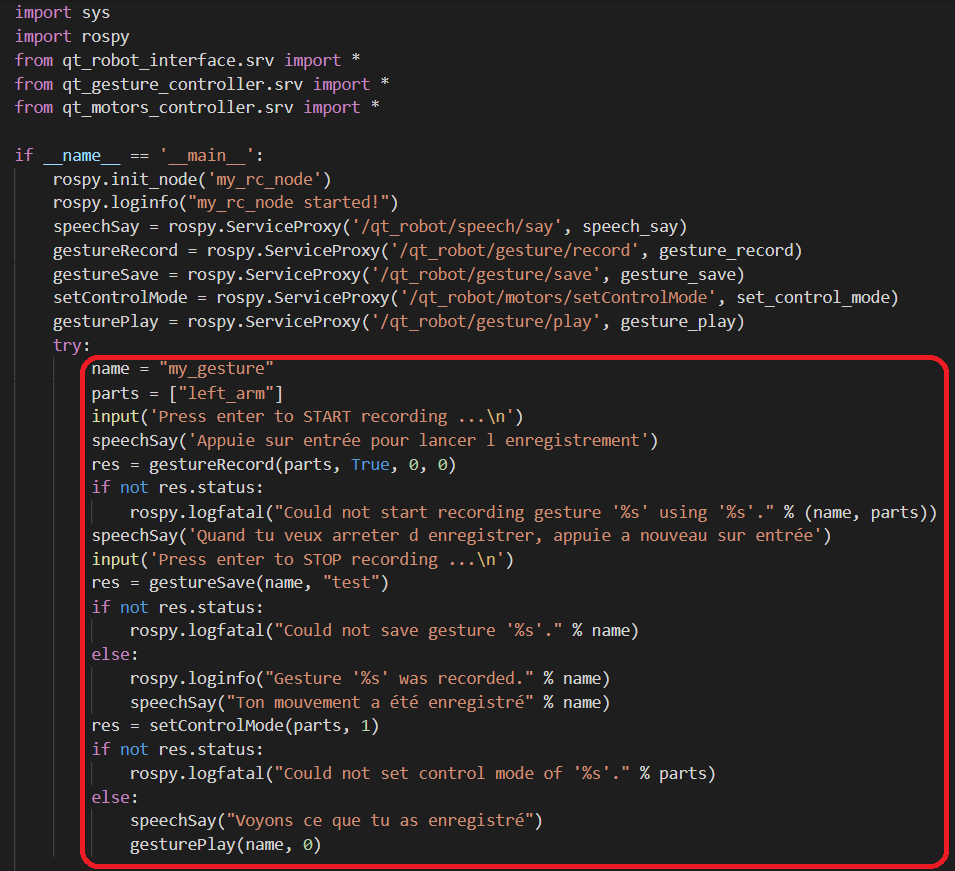
\includegraphics[width=\textwidth]{Figures/qtrobotscript4mouvement.png}
\captionof{figure}{Python script left arm movements}
\end{minipage}%
\hfill
\begin{minipage}{.33\textwidth}%
In our script, we record a movement for the left arm. When we launch the recording, it unlocks and we can start moving the arm and make any movement we like. When finished, press enter to stop recording. The robot will then reproduce the movement.\\
\end{minipage}%

\section{VR}
\subsection{Modeling}
\subsubsection{Blender}
\begin{minipage}{.5\textwidth}%
We began by modeling the QTrobot using Blender. We explored the functionalities of this 3D modeling tool and tried to faithfully recreate the robot's appearance. Unfortunately, we encountered a number of difficulties and didn't achieve the desired results. Proportions and details didn't exactly match those of the real QTrobot, limiting the accuracy of the virtual representation.\\
\end{minipage}%
\hfill
\begin{minipage}{.35\textwidth}%
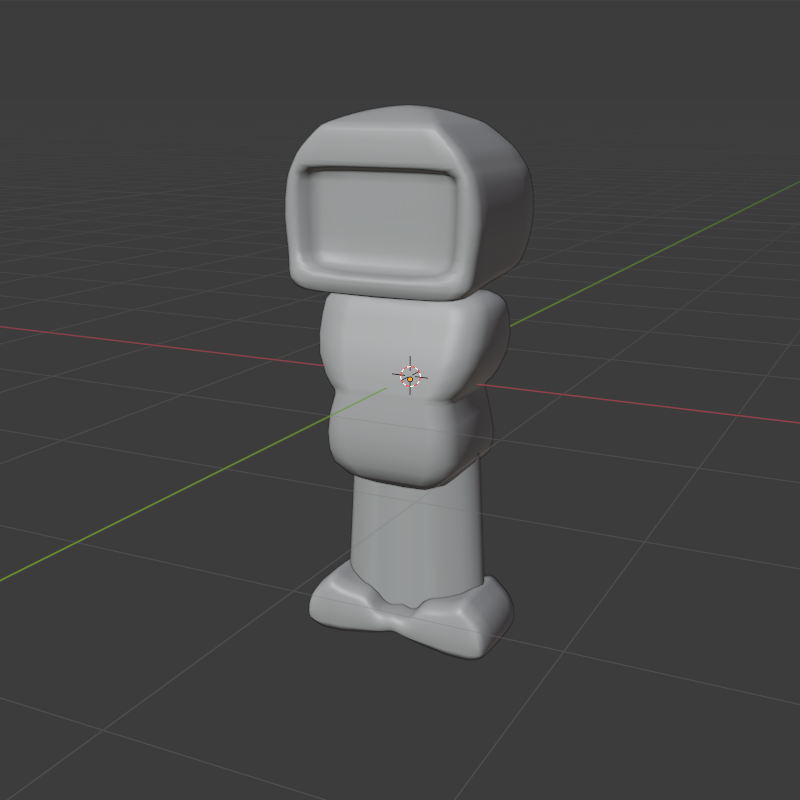
\includegraphics[width=\textwidth]{Figures/QT3D_blender.png}
\captionof{figure}{QTrobot blender}
\end{minipage}%
\\
\subsubsection{Polycam}
\begin{minipage}{.5\textwidth}%
We persevered and decided to explore other options. That's when we turned to PolyCam. This solution enabled us to model the QTrobot much more successfully. Thanks to PolyCam's photogrammetry technology, we were able to capture the robot's dimensions and features with even greater precision. The end result was a virtual representation more faithful to reality, offering an immersive and realistic experience for virtual reality users.\\
\end{minipage}%
\hfill
\begin{minipage}{.35\textwidth}%
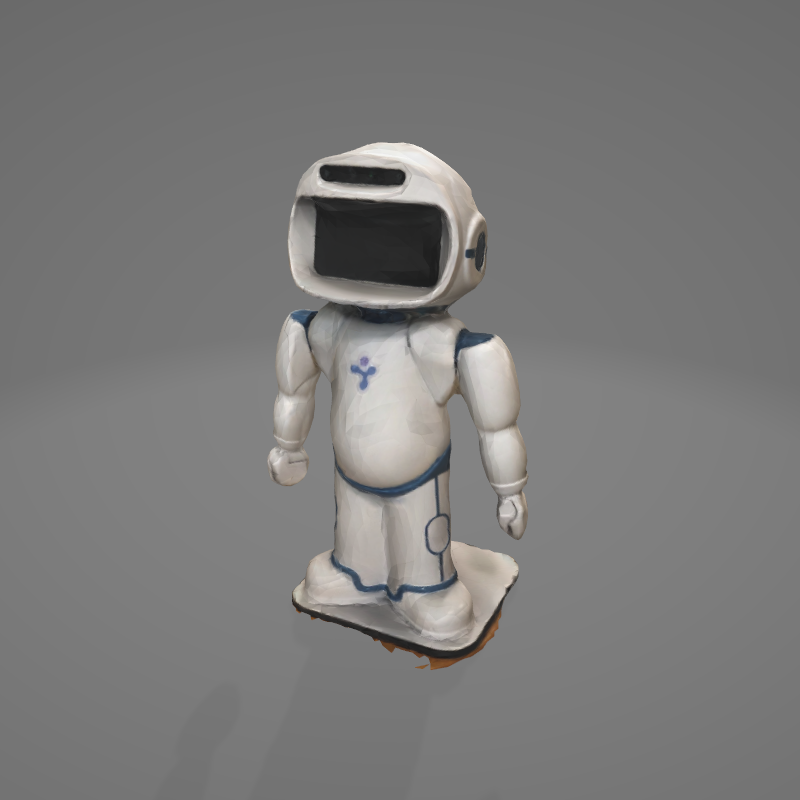
\includegraphics[width=\textwidth]{Figures/QT3D_photogrametrie.png}
\captionof{figure}{QTrobot polycam}
\end{minipage}%
\\


\subsection{Setting up the Unity project}
Once the robot model has been exported, it needs to be integrated into a 3D scene and a VR camera added so that the user can observe the scene. To share code, Unity doesn't (simply and free of charge) allow projects to be synchronized on Git. We therefore had to use the collaboration system developed by Unity: PlastiSCM. To integrate VR into Unity, we use OVR (Oculus Virtual Reality), a virtual reality platform developed by Oculus..\\
\\
For some years now, Meta has been heavily involved in the field of virtual reality, developing tools to integrate VR into a wide range of areas. There's a component that can be integrated into Unity to configure and manage virtual reality functionalities, called OVR Manager. Thanks to OVR Manager, we were able to take advantage of the tools and functionalities of the Oculus platform to create an immersive and realistic virtual reality experience. \\ 

\begin{figure}[!h]
\centering
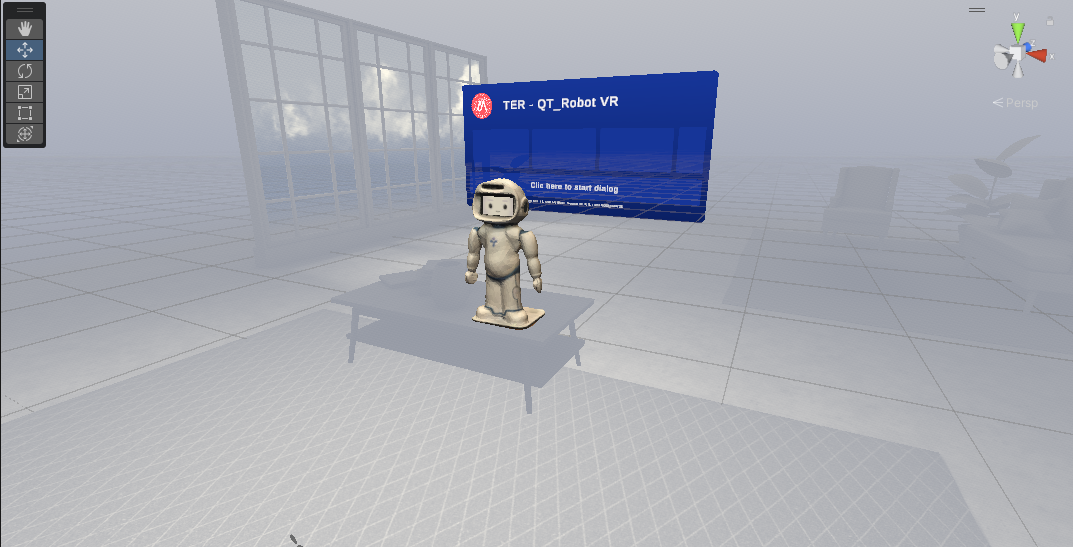
\includegraphics[height=7cm]{Figures/Scene_3D.png}
\caption{Screenshot of the final scene}
\end{figure}

\subsubsection{Dialogue}
The integration of Meta's API also enabled us to record a response from the user. Indeed, before we came up with the idea of the Wizard of Oz experience, it was based on a simple dialogue between the robot and the user. We chose to detect the user's voice in order to retrieve the text and pass it to ChatGPT using the OpenAI API to retrieve a response to give to the user. After a few tests, we noticed that users' feelings depended very much on the answer given by ChatGPT, which would have biased the results of the experiment. \\
\\
To ensure a match between the robot and VR experience, we pre-recorded the QT Robot's answers and played them back in the Unity scene. When the experimenter plays a question, the recording corresponding to the question is played.\\

\begin{figure}[!h]
\centering
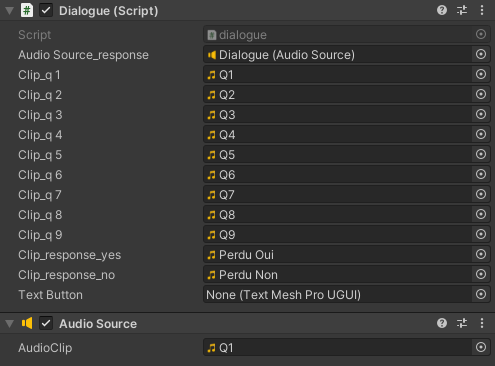
\includegraphics[height=7cm]{Figures/UnityDialogue.png}
\caption{Visualizing attributes on Unity}
\end{figure}

\begin{figure}[!h]
\centering
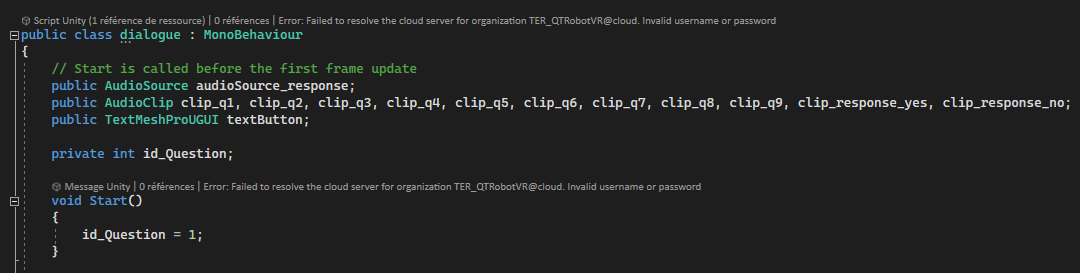
\includegraphics[height=3.5cm]{Figures/VSDialogue.png}
\caption{Declaring attributes in the script}
\end{figure}

\newpage
Here's how the experience is managed on the Unity side, with the example of launching responses. In figure 3.14, variables of type "AudioClip" have been declared and can be assigned in the Unity editor, as they are declared as "public". The rest of the script takes care of launching the desired audio file in the source audio, which is set to be played on the VR headset using the OVR Manager.